\documentclass[a4paper,floatfix,nofootinbib]{article}
\usepackage{amsmath,amssymb}
\usepackage{graphicx}
\usepackage{listings}
\graphicspath{ { . } }

\title{Homework 1}
\author{Sierra LaRosa}

\begin{document}

\maketitle

\section*{Problem 2.1}
Suppose you flip four fair coins:

\begin{itemize}
    \item Make a list of all possible outcomes.
    \item Make a list of all the different macro states and their probablilities.
    \item Compute the multiplicity of the macrostates using the the Choose function $N \choose n$
\end{itemize}

\subsection*{a}
List of all possible outcomes:
\begin{itemize}
    \item HHHH
    \item HHHT
    \item HHTH
    \item HTHH
    \item HTHH
    \item THHH
    \item HHTT
    \item HTHT
    \item HTTH
    \item THHT
    \item TTHH
    \item HTTT
    \item THTT
    \item TTHT
    \item TTTH
    \item TTTT
\end{itemize}

\subsection*{b}
List of all different macro states and their probabilities:

\begin{itemize}
    \item Four heads: 1 outcome has a probability of $1/16$ chance.
    \item Three heads: 4 outcomes has a probability of $4/16$ = $1/4$ chance.
    \item Two heads: 6 outcomes has a probability of $6/16$ = $3/8$ chance.
    \item One head: 4 outcomes has a probability of $4/16$ = $1/4$ chance.
    \item No heads: 1 outcome has a probability of $1/16$ chance.
\end{itemize} 

\subsection*{c}
Calculating the probability of each macrostate is as follows:

\begin{equation}
    \binom{4}{n} = \frac{ 24 }{ n! \times \left( 24 - n \right) \,! }
\end{equation}

Where $n$ is the number of coins that landed on heads. So for this


\begin{itemize}
    \item Four heads:
        \begin{align*}
            \binom{4}{4} &= \frac{ 24 }{ 4! \times \left( 4 - 4 \right) \,! } \\
            &= \frac{ 24 }{ 4! \times \left( 0 \right) \,! }                   \\
            &= 1
        \end{align*}

    \item Three heads:
        \begin{align*}
            \binom{4}{3} &= \frac{ 24 }{ 3! \times \left( 4 - 3 \right) \,! } \\
            &= \frac{ 24 }{ 3! \times \left( 1 \right) \,! } \\
            &= 4
        \end{align*}

    \item Two heads:
        \begin{align*}
            \binom{4}{2} &= \frac{ 24 }{ 2! \times \left( 4 - 2 \right) \,! } \\
            &= \frac{ 24 }{ 2! \times \left( 2 \right) \,! } \\
            &= 6
        \end{align*}

    \item One head:
        \begin{align*}
            \binom{4}{1} &= \frac{ 24 }{ 1! \times \left( 4 - 1 \right) \,! } \\
            &= \frac{ 24 }{ 1! \times \left( 3 \right) \,! } \\
            &= 4
        \end{align*}

    \item No heads:
        \begin{align*}
            \binom{4}{0} &= \frac{ 24 }{ 0! \times \left( 4 - 0 \right) \,! } \\
            &= \frac{ 24 }{ 0! \times \left( 4 \right) \,! } \\
            &= 1
        \end{align*}
\end{itemize} 

\section*{Problem 2.2}
Suppose you flip 20 coins:

\subsection*{a}
How many possible outcomes (microstates) are there? Coins can be considered a binary state, i.e. an $N$ number of coins is: $2^N$. Therefore ther are $2^{20} = 1048576$ possible outcomes (microstates) when flipping 20 coins.

\subsection*{b}
What is the probability for getting the flip sequence of: HTHHTTTHTHHHTHHHHTHT in exactly that order? It can be assumed that the probabily of a state of a binary state like a coin is $1/2^N$ where $N$ is the how many coins are being flipped. The question only asks for the microstate and not the macrostate of 12 head flips and 8 tail flips. Therefore the probability of getting the flip sequence of HTHHTTTHTHHHTHHHHTHT in exactly that order is $(1/2)^20 = 1/1048576$.

\subsection*{c}
What is the probability of getting 12 heads and 8 tails in any order? In this case the question asks in more explicit terms: what is the probability of the macrostate having 12 heads and 8 tails in the outcome, or what is $\Omega(12)/2^{20}$. 
\begin{align*}
    \Omega(12)/2^{20} &= \frac{\binom{20}{12}}{2^{20}} \\
        &= \frac{ 20! }{ 12! \times \left( 8 \right) \,! } \times \frac{ 1 }{ 2^{20} } \\
        &= 125970 \times \frac{ 1 }{ 2^{20} }   \\
        &= \frac{ 62985 }{ 524288 } \ \textrm{or} \ 12.0134\%
\end{align*}

\section*{Problem 2.3}
Suppose you flip 50 coins:

\subsection*{a}
How many possible outcomes are there?
There are $2^{50} = 1125899906842624$ possible outcomes when flipping 50 coins.

\subsection*{b}
How many ways are there of getting exactly 25 heads and 25 tails?
There are ${50 \choose 25} = 2118760$ ways of getting exactly 25 heads and 25 tails.

\subsection*{c}
What is the probability of getting exactly 25 heads and 25 tails? For the following excercises, refer to the method as outlined in \textbf{Problem 2.2b} as these caculations are identical except in inputs. The probability of getting exactly 25 heads and 25 tails is $\frac{{50 \choose 25}}{2^{50}} = 11.228\%$.

\subsection*{d}
What is the probability of getting exactly 30 heads and 20 tails? The probability of getting exactly 30 heads and 20 tails is ${50 \choose 30} * \left(\frac{1}{2}\right)^{30} * \left(\frac{1}{2}\right)^{20} = 4.19\%$.

\subsection*{e}
What is the probability of getting exactly 40 heads and 10 tails? The probability of getting exactly 40 heads and 10 tails is ${50 \choose 40} * \left(\frac{1}{2}\right)^{40} * \left(\frac{1}{2}\right)^{10} = 9.12 \times 10^{-6} \%$.

\subsection*{f}
What is the probability of getting exactly 50 heads and 0 tails? The probability of getting exactly 50 heads and 0 tails is ${50 \choose 50} * \left(\frac{1}{2}\right)^{50} = 8.88 \times 10^{-16} \%$.

\subsection*{g}
Make a plot of the probability of getting n heads, as a function of n.
Using a simple python program: 
\begin{lstlisting}
import matplotlib.pyplot as plt
import numpy as np
from math import comb

# Define the number of coins
n = 50

# Create an array of possible number of heads
heads = np.arange(0, n+1)

# Calculate the probability of getting n heads
prob = [comb(n, h) * (1/2)**h * (1/2)**(n-h) for h in heads]

# Create the plot
plt.plot(heads, prob)
plt.xlabel('Number of Heads')
plt.ylabel('Probability')
plt.title(f'Probability of Getting n Heads for {n} Coins')
plt.show()
\end{lstlisting}

\newpage

This generates the following plot:
\begin{figure}[hH]
    \centering
    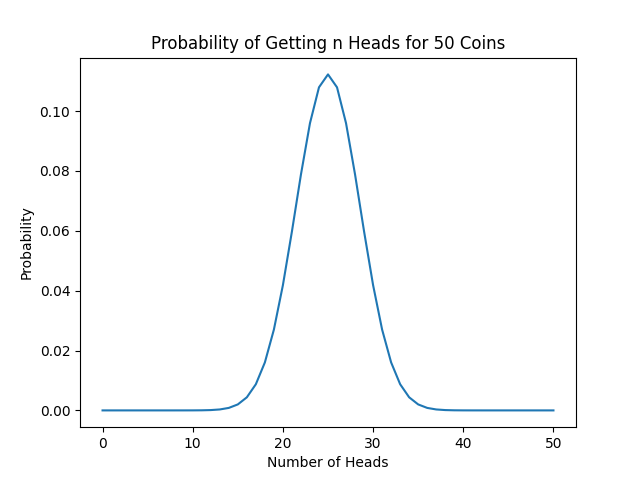
\includegraphics[width=0.75\textwidth]{Figure_1.png}
    \caption{Probability of Getting n Heads for 50 Coins}
\end{figure}

\end{document}
